\section{Massive activations in stage~3}
\label{app:massive-activations}

\Cref{sec:massive_activations} summarises the outliers found in stage~3 of ConvNeXt and Swin.
Here we detail how they are identified, how we ablate the ConvNeXt channel and what their kinematics look like.
Throughout, we use ``massive activation'' loosely for channels or tokens that exceed all others by more than an order of magnitude.
On the shared and untied ConvNeXt the stage-3 exit also meets the numerical criterion of \citet{sun2024massiveactivationslargelanguage} (magnitude above $100$ and about $10^3$ times the median), although here the dominant channel is large at every position rather than at a few tokens, a pattern closer to the uniformly large feature dimension that \citet{sun2024massiveactivationslargelanguage} report for MAE ViTs and do not count as massive: at every spatial position $\max_c|x_c|>100$, and the median over positions of $\max_c|x_c|/\mathrm{median}_c|x_c|$ is about $1.1{\times}10^3$ (shared, $N{=}500$) and $1.3{\times}10^3$ (untied, $N{=}500$).
In Swin the corner tokens fail that channel-wise test (ratios of about $16$), so the label there refers only to their outlying L2 norms.

\paragraph{Detection.}
On the shared ConvNeXt we integrate the native stage-3 schedule ($D{=}9$, $\Delta t{=}1$, Euler) on a single ImageNet validation image and rank the $384$ channels by the Frobenius norm $\|x_c\|_F$ of the stage-3 state just before LayerNorm and downsampling.
Channel~$236$ dominates by more than an order of magnitude ($\|x_{236}\|_F\approx 3.6{\times}10^3$ vs.\ $\approx 1.4{\times}10^2$ for the runner-up; \cref{fig:massive-norms}).
The same index remains the top channel under the refined schedule ($R{=}10$, $D{=}90$, $\Delta t{=}0.1$), so the outlier is not an artefact of the unit-step discretisation.
An analogous ranking on the untied ConvNeXt-T likewise isolates one channel of comparable relative size, channel~$195$; ResNet stage~3 has no channel of this dominance.

\begin{figure}[t]
    \centering
    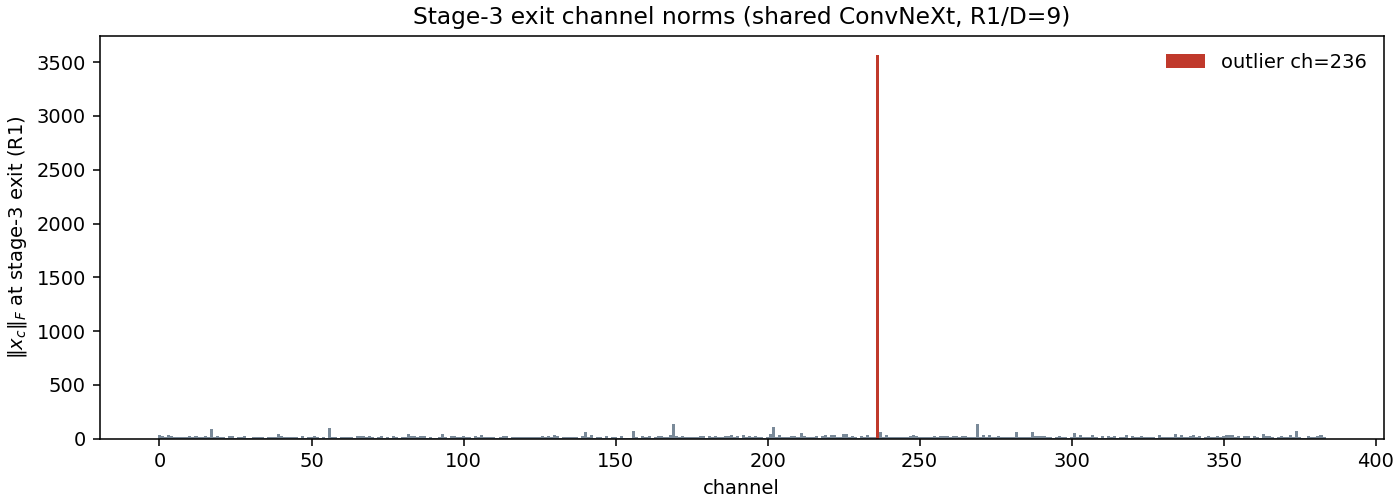
\includegraphics[width=\linewidth]{figures/massive_channel_norms.png}
    \caption{Stage-3 exit channel norms on the shared ConvNeXt ($R{=}1$, $D{=}9$). Channel~$236$ (red) is the massive activation used in the ablations below.}
    \label{fig:massive-norms}
\end{figure}

\paragraph{Zeroing protocol.}
To test functional importance we re-run the full ImageNet validation pass while forcing the selected channel to zero after \emph{every} residual step of stage~3 (stem and stages~1--2,~4 are untouched).
We compare three conditions under both the native ($R{=}1$) and refined ($R{=}10$) shared schedules, always at the trained horizon $T{=}9$:
(i)~baseline, no channel forced;
(ii)~outlier, channel~$236$ zeroed;
(iii)~random controls, each of $20$ channels drawn uniformly from $\{0,\ldots,383\}\setminus\{236\}$ (seed~$0$) zeroed independently.
\Cref{tab:app-massive-zero} reports top-1 and cross-entropy; \cref{fig:massive-delta-loss} shows the corresponding $\Delta$loss histogram.
Zeroing the outlier costs about $12.5$~pp of top-1 and raises the loss by $\approx 0.69$, while every random channel stays within $0.3$~pp and $\Delta\mathrm{loss}\le 0.02$.
The drop is essentially unchanged from $R{=}1$ to $R{=}10$, so the channel remains critical under refinement.

\begin{table}[t]
    \centering
    \caption{Shared ConvNeXt-T ImageNet validation when zeroing one stage-3 channel after every residual step. Random: mean and range over $20$ channels.}
    \label{tab:app-massive-zero}
    \small
    \setlength{\tabcolsep}{3pt}
    \resizebox{\linewidth}{!}{%
    \begin{tabular}{llrrr}
        \toprule
        $R$ & condition & top-1 (\%) & loss & $\Delta$loss \\
        \midrule
        1  & baseline            & 80.34 & 0.896 & -- \\
        1  & zero ch~$236$       & 67.81 & 1.595 & $+0.699$ \\
        1  & zero random ($n{=}20$) & $80.25$ [$80.05$,\,$80.38$] & -- & $\le 0.018$ \\
        \midrule
        10 & baseline            & 80.14 & 0.904 & -- \\
        10 & zero ch~$236$       & 67.59 & 1.590 & $+0.686$ \\
        10 & zero random ($n{=}20$) & $80.11$ [$79.85$,\,$80.18$] & -- & $\le 0.019$ \\
        \bottomrule
    \end{tabular}%
    }
\end{table}

\begin{figure}[t]
    \centering
    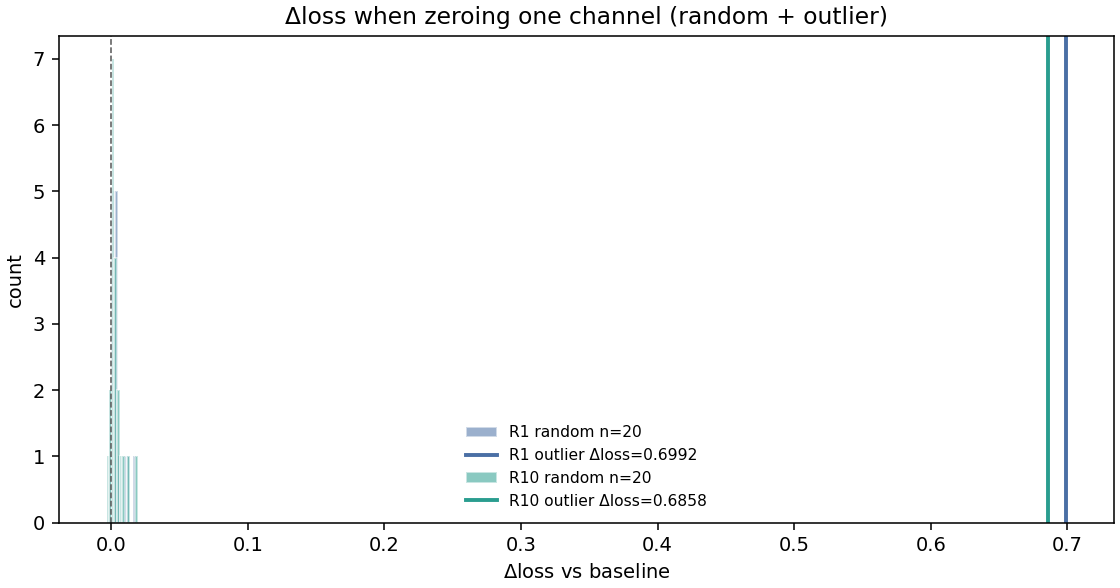
\includegraphics[width=0.85\linewidth]{figures/massive_delta_loss_hist.png}
    \caption{$\Delta$loss vs.\ baseline when zeroing one stage-3 channel on the shared ConvNeXt. Random channels ($n{=}20$ per $R$) cluster near zero; the outlier (vertical lines) sits near $\Delta\mathrm{loss}\approx 0.7$ for both $R{=}1$ and $R{=}10$.}
    \label{fig:massive-delta-loss}
\end{figure}

These numbers show that the trained network relies on this channel, but not that a massive channel is necessary: zeroing it also removes its contribution to the LayerNorm statistics at every spatial position and therefore rescales all other channels.

\paragraph{Phase portraits.}
\Cref{fig:massive-phase} plots, for every stage-3 channel, the trajectory of spatial means $(\mathrm{mean}_{H,W}(x_d),\,\mathrm{mean}_{H,W}(h_d))$ over $T{=}9$ at $\Delta t{=}0.01$ ($N{=}500$ validation images).
In the shared model the outlier traces a smooth arc: the residual mean $\mathrm{mean}(h)$ rises then falls while the state mean $\mathrm{mean}(x)$ keeps growing, matching the early acceleration and late velocity drop reported in the main text.
In the untied ConvNeXt-T the dominant channel advances in a block-wise sawtooth and moves away from the origin, its magnitude growing with negative sign: its velocity decays within most blocks and jumps at every block boundary.
In both models the spatial means of the remaining $383$ channels stay close to the origin.
This dominance is why we exclude the outlier channel when computing the trajectory-geometry metrics of the main text; the forward pass itself is left unchanged.

\begin{figure*}[t]
    \centering
    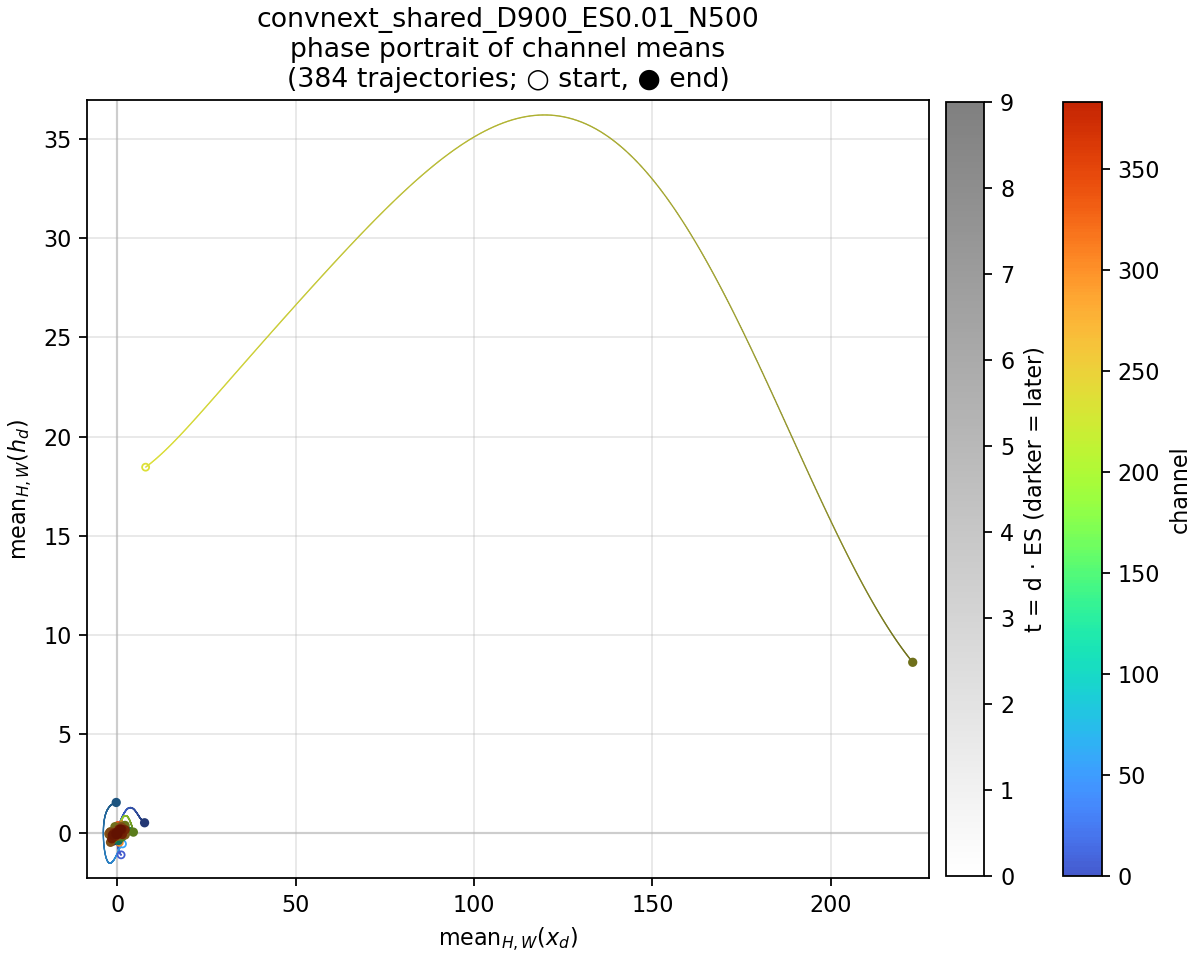
\includegraphics[width=0.49\textwidth]{figures/massive_phase_shared.png}%
    \hfill
    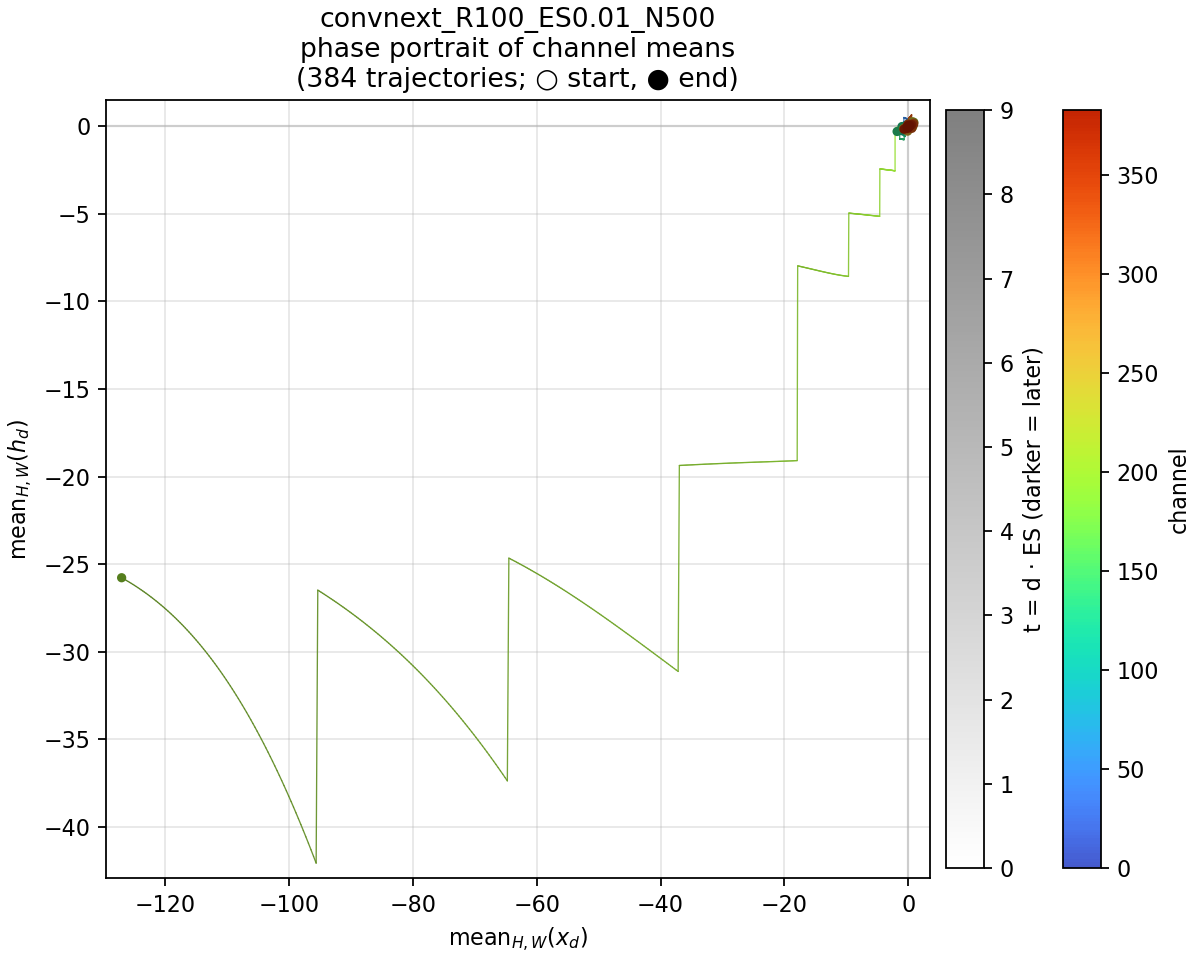
\includegraphics[width=0.49\textwidth]{figures/massive_phase_convnext.png}
    \caption{Phase portraits of stage-3 channel means $(\mathrm{mean}_{H,W}(x_d),\,\mathrm{mean}_{H,W}(h_d))$ over $T{=}9$ ($\Delta t{=}0.01$, $N{=}500$ images).
    \textbf{Left:} shared ConvNeXt ($D{=}900$).
    \textbf{Right:} untied ConvNeXt-T ($R{=}100$).
    One channel reaches spatial means more than an order of magnitude larger than those of the remaining 383 channels, which stay close to the origin.}
    \label{fig:massive-phase}
\end{figure*}

\paragraph{Swin.}
In Swin-T the outliers are concentrated in tokens rather than channels, so means hide them: averaging over channels cancels coordinates of opposite sign, and averaging over positions dilutes four tokens among $196$.
We therefore plot, for each stage-3 position, the norm over channels of the state $\|x_d\|_C$ against that of the residual $\|h_d\|_C$ (\cref{fig:swin-massive}, left).
The four corner tokens end the stage with norms of about $500$ to $600$, whereas the median norm over the remaining $192$ positions is $23$.
Most of this growth happens in the last two of the six blocks, where the norm increases by almost the full integral of $\|h_d\|_C$. Since the per-step change of the norm is at most $\Delta t\,\|h_d\|_C$, with equality only when $h_d$ is parallel to $x_d$, these blocks amplify the corner tokens along their own direction, and the tokens are still growing when the stage ends.
Averaged over $500$ images, the corner tokens still show large values in the same few channels with the same signs (\cref{fig:swin-corner-slice}), which suggests a mechanism largely independent of the input.
Averaging over positions instead (\cref{fig:swin-massive}, right), one channel grows above the rest in a block-wise sawtooth similar to that of the untied ConvNeXt, but its final spatial mean is only about three times that of the next largest channel.

\begin{figure*}[t]
    \centering
    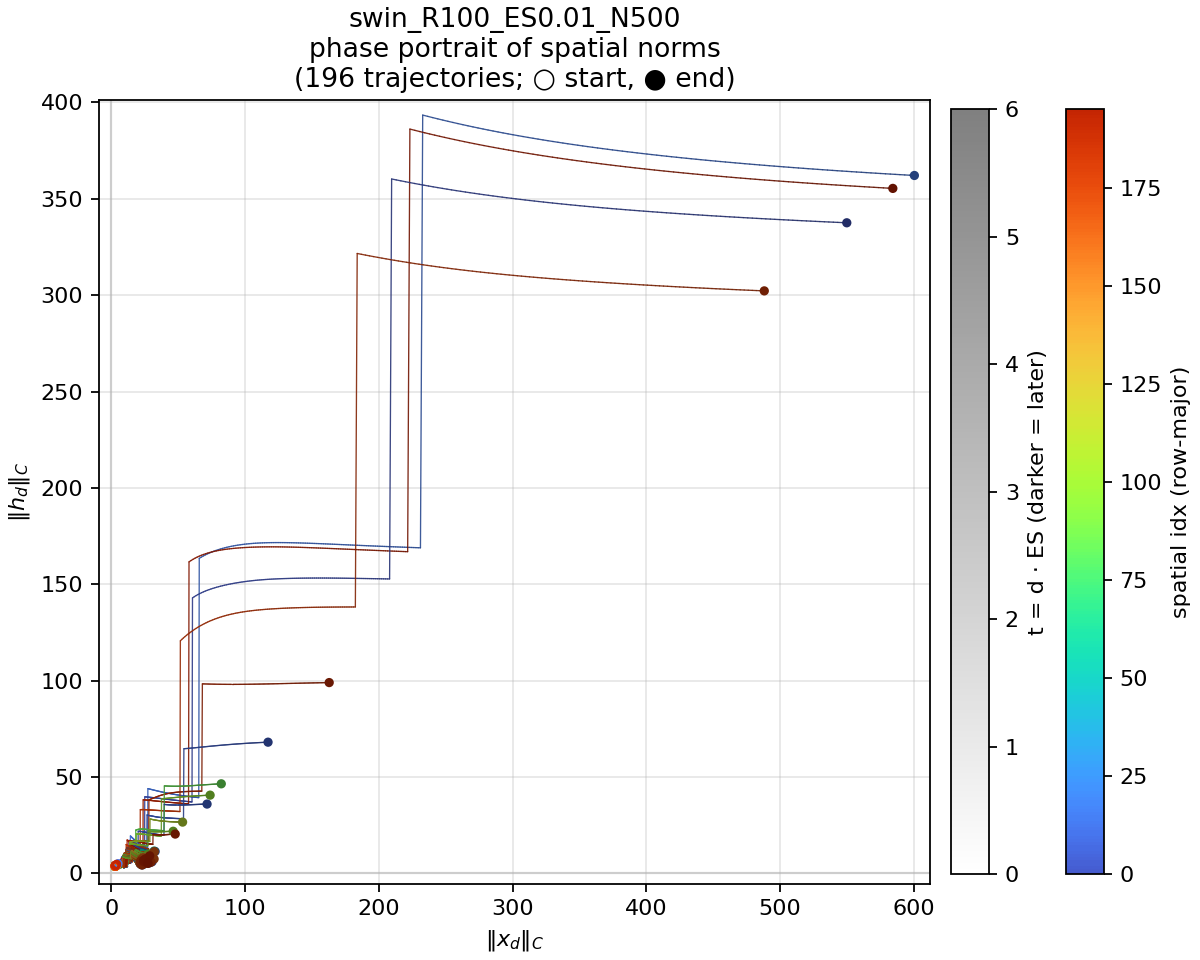
\includegraphics[width=0.49\textwidth]{figures/swin_phase_token_norms.png}%
    \hfill
    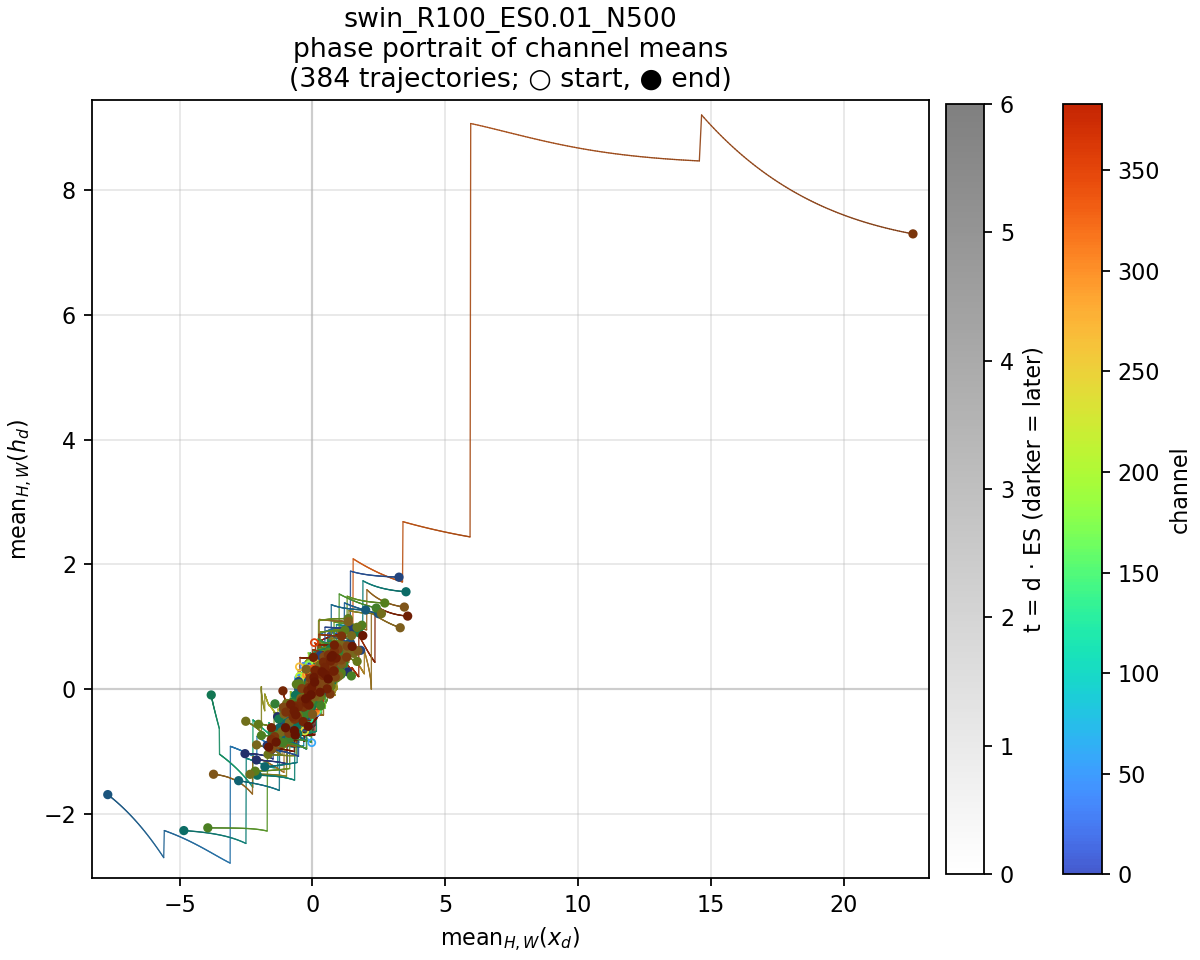
\includegraphics[width=0.49\textwidth]{figures/swin_phase_channel_means.png}
    \caption{Swin-T stage~3 ($R{=}100$, $\Delta t{=}0.01$, $T{=}6$, $N{=}500$ images).
    \textbf{Left:} one trajectory per spatial position, $(\|x_d\|_C,\,\|h_d\|_C)$; the four outlying trajectories are the corner tokens.
    \textbf{Right:} one trajectory per channel, $(\mathrm{mean}_{H,W}(x_d),\,\mathrm{mean}_{H,W}(h_d))$; one channel grows above the rest in a block-wise sawtooth.}
    \label{fig:swin-massive}
\end{figure*}

\begin{figure*}[t]
    \centering
    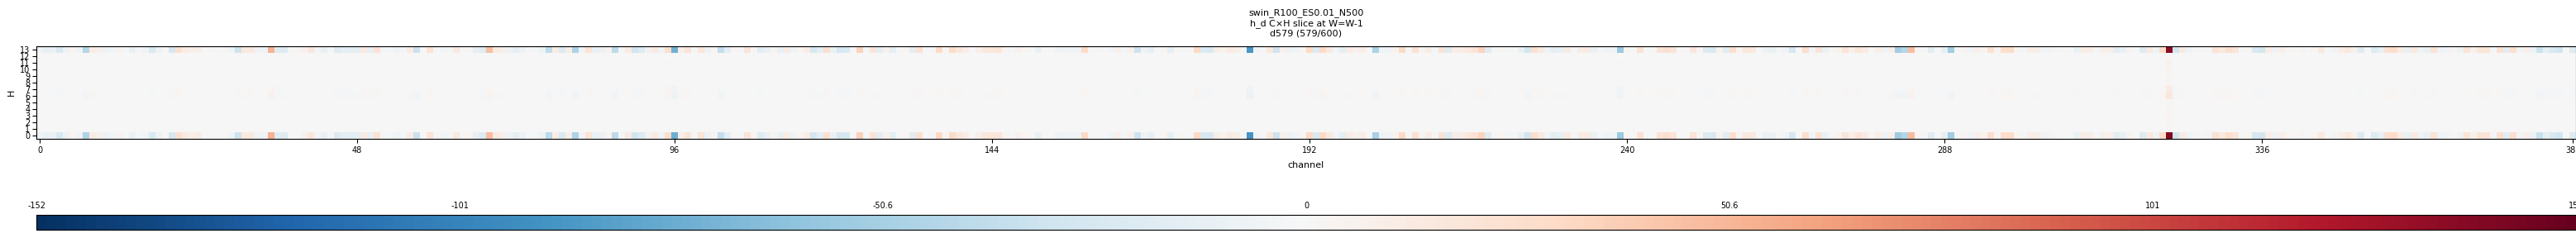
\includegraphics[width=\textwidth]{figures/swin_corner_slice_W13.png}\\[0.5em]
    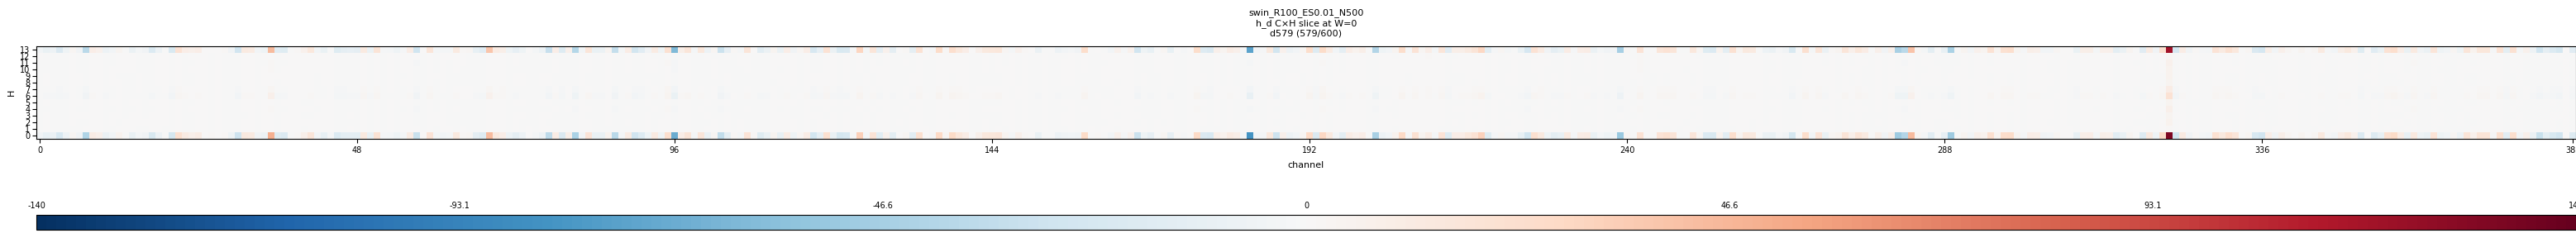
\includegraphics[width=\textwidth]{figures/swin_corner_slice_W0.png}
    \caption{Residual $h_d$ of Swin-T stage~3 at step $d{=}579$ (last block), averaged over $500$ images and shown as channel by height slices at the last column (\textbf{top}) and at $W{=}0$ (\textbf{bottom}). Rows $0$ and $13$ of each panel are the four corner tokens, which share the same dominant channels and signs.}
    \label{fig:swin-corner-slice}
\end{figure*}

\paragraph{Interpretation.}
Massive activations arise in pre-norm residual blocks and are suppressed when the
vector-wise normalisation is replaced by an element-wise one~\citep{pmlr-v306-sun26d}.
This fits what we see: ConvNeXt and Swin normalise each position across channels with
LayerNorm, whereas BatchNorm~\citep{ioffe2015batchnorm} in ResNet normalises each
channel independently; ResNet stage~3 shows no outlier.
A channel-concentrated pattern has also been reported for diffusion
transformers~\citep{gan2025ditf}.
In language models massive activations are injected by a few early blocks and then stay
nearly constant until late blocks remove them, acting as fixed bias
terms~\citep{sun2024massiveactivationslargelanguage,pmlr-v306-sun26d}.
The ConvNeXt channel instead evolves throughout the stage with the same kinematic
profile as the rest of the state (\cref{fig:massive-phase}).
In the shared model the explicit parameters are identical at every step, so the block
can access depth only through the state.
We conjecture that this channel provides that signal, as an autonomous system can
emulate a non-autonomous one by carrying time as an extra state
variable~\citep{strogatz2015nonlinear}, which time-dependent Neural ODEs implement
explicitly~\citep{dupont2019augmented}.
Our observations are consistent with this reading but do not establish it.

\paragraph{Open questions.}
Two tests would clarify the role of the ConvNeXt channel.
Following the set-to-mean intervention of \citet{sun2024massiveactivationslargelanguage}, replacing it by its mean over images at the same step, instead of zero, would also approximately preserve the LayerNorm statistics and thus separate the effect of the channel from that of the renormalisation.
Tracking the ratio between the channel and the RMS of the remaining channels along depth separates the two readings of \cref{sec:massive_activations}: as an implicit parameter the ratio should stay roughly constant, whereas as a depth signal it should vary systematically with $t$, particularly in the shared model.
A finer characterisation of the Swin corner tokens, including how they evolve after stage~3, is left for future work.

\FloatBarrier
